\setchapterpreamble[u]{\margintoc}
\chapter{AI-Enabled Mass Destruction}
\labch{introduction}

\textit{There is little doubt that AI will contribute to profound transformations over the next decades. At its best, the technology has the potential to release us from mundane work and create a utopia in which all time is leisure time. At its worst, World War III might be fought by armies of superintelligent robots. But they won’t be led by HAL, Skynet or their newer AI relatives. Even in the worst case, the robots will remain under our command, and we will have only ourselves to blame.} Anthony Zador, Yann LeCun 2019 \cite{dontfearterminator}


\section{The AI Renaissance}

Technology often finds its first adopters among those who can afford it and foresee its potential. Artificial Intelligence (AI) is no exception, with its early applications dating back several decades, notably in the financial industry. Hedge funds and investment banks identified the value of AI and started using it for trading and portfolio management.

Renaissance Technologies, a hedge fund founded by mathematician James Simons, exemplifies the early adoption of AI. Since 1978 the company has used AI to predict market movements and optimize trading strategies. By employing highly skilled PhDs known as "quants" to develop algorithms and AI models, Renaissance Technologies has become one of the most successful hedge funds in history.

As AI gained traction, tech giants like Google and Microsoft began investing in their own quants. These experts were tasked with using AI to address a wide range of challenges, from refining search algorithms to enhancing language processing capabilities. Much of this research was made public, allowing the broader community to benefit from these advancements. AI-enabled products became visible to more visible to consumers, and AI tooling became very accessible to developers. Online advertising advertising became a highly visible industry where AI is able to analyze user behavior and target ads with remarkable precision.

\begin{pdf}
\begin{marginfigure}[-5.5cm]
    
\includegraphics{purplehair}
        \caption{"Portrait of a beautiful young woman with purple hair looking into the camera. Associated press. Photojournalism. Street photography." made with Stable Diffusion 2.1 try it yourself at \url{https://stability.ai/}}
        \labfig{purplehair}
\end{marginfigure}
\end{pdf}

The accessibility of AI technology has increased, thanks in part to open-source projects that enable individuals and smaller organizations to tap into its power. This democratization of AI has ignited a wave of innovation, with developers worldwide contributing to the AI renaissance. Developments in AI have turned a corner; large open-source datasets coupled with cheap computing power and powerful open-source development tools have taken AI out of the realm of expensive private enterprise into a new era, where companies give away large and valuable models under strong public licences (like Stable Diffusion from StabilityAI, LLaMA from facebook) and the most innovative companies operate as large non-profit or limited-profit entities (like OpenAI, the creators of ChatGPT).   


The world of open AI acknowledges that training data is valuable, but realizes that especially on the internet, information wants to be free.  The risks of data theft and unauthorized use have escalating, and the industry is simultaneously having its "iPhone moment" with the advent of ChatGPT, and its "Napster Moment" with the public release of large generative models trained on copyrighted content\sidecite{copyrighteconocmist}. Companies and individuals are striving to protect their intellectual property while others look for ways to exploit it, but if the past is a guide copyright holders are likely to lose out, as the ability to capture income from from copywritten content moves from content creators and to content distributors, namely large cloud computing companies that run AI models at scale.

This situation sets the stage for an AI copyright battle looming on the horizon. As the distinction between proprietary and open-source information blurs, the question of who owns AI-generated content becomes increasingly important. Governments, corporations, and individuals are all grappling with the legal and ethical implications of AI and its widespread adoption. When one considers that AI models themselves are content that can be modeled and stolen, one can get a glimpse of the full destructive and transfomative power of AI. AI doesn't just allow you to benefit from copywritten text and images and create your own that you can distribute, AI also allows you to copy the multibillion dollar models that researchers at Google, Microsoft and Facebook have made and modify and distribute them as long as you have the technical know-how and a big enough computer to run the models. The AI renaissance is breaking traditional business models and also breaking the business models of its creators almost as soon as it is released. Like many transformative technologies, AI is shrinking the market, making things cheap for everyone, and capturing market share.

\begin{pdf}
\begin{marginfigure}[-5.5cm]
    
\includegraphics{waffleburger}
        \caption{"a delicious cheesebuger made with waffles instead of a bun and covered with rasperry jam" made with Stable Diffusion 2.1}
        \labfig{waffleburger}
\end{marginfigure}
\end{pdf}

\section{AI Shrinks the Market and Takes Market Share}

The "Software Paradox" posits that as software becomes more open, it tends to shrink markets while capturing most of the market share. This phenomenon can be observed in the current state of AI, particularly with the advent of open-source AI. As AI technologies become more sophisticated and widespread, they are reducing the need for human labor in many markets, and bring the cost of creation down significantly across industries.\sidecite{OGrady2015}

One key aspect of AI's impact on the market is its ability to automate repetitive and mundane tasks, allowing humans to focus on more complex and creative aspects of their work. This not only streamlines processes but also has the potential to improve the overall quality of work. With AI handling the less desirable tasks, human workers can concentrate on utilizing their unique skills and expertise, resulting in better outcomes and higher value-added work.

The rise of open-source AI further accelerates this trend, making advanced AI tools and algorithms accessible to a broader range of individuals and organizations. As these powerful tools become more widely available, businesses across various industries will find it increasingly difficult to justify the cost of employing human workers for tasks that can be more efficiently completed by AI. This shift will result in a smaller job market for those specific tasks, with AI taking the majority of the market share.

However, the shrinking of specific labor markets does not necessarily mean the eradication of all human work. Instead, it presents an opportunity for the workforce to adapt and focus on roles that are complementary to AI systems. This could involve tasks that require empathy, complex problem-solving, or human intuition, which are areas where AI currently struggles to excel.

\section{The Other Economy, the One Without AI}

As AI revolutionizes various sectors of the economy, there's another economy that remains untouched by AI's transformative effects. This other economy is characterized by heavily regulated industries that often resist technological innovation, resulting in stagnating growth and rising costs for consumers\sidecite{andreesenunemp}.

In many places, AI is practically illegal. This is partly due to consumers, professional organizations and governments struggling to keep up with the rapid pace of technological advancements, leading to a lack of understanding and appropriate regulations \sidecite{lawmakersny}. Additionally, public opinion remains skeptical about the widespread adoption of AI, as evidenced by polls\sidecite{morningconsult}\sidecite{monmouthai}. This skepticism is not helped by stories of software developers becoming emotionally attached to AI chatbots\sidecite{googlenerd}.

The contrast between sectors that embrace AI and those that resist it highlights a growing divide in the economy. In industries where AI is allowed to flourish, technological innovation drives down prices and increases product quality, leading to a more efficient market. However, heavily regulated sectors that resist AI adoption experience rising costs and stagnating growth, ultimately consuming a larger share of the economy.

This phenomenon is exacerbated by the emotional interplay between production and consumption. As consumers, we tend to become frustrated with price increases in the heavily regulated sectors. On the other hand, as producers, we may feel threatened by technological disruption in industries that embrace AI. This dichotomy demonstrates the inherent conflict between the desire for stability in the economy and the need for innovation and progress.

As the regulated, non-technological sectors continue to grow as a percentage of GDP, the economy may ultimately become dominated by these stagnating industries. In such a scenario, the full potential of AI and other advanced technologies may never be realized. This highlights the importance of addressing regulatory barriers, fostering public understanding, and promoting AI adoption in industries that have yet to embrace its potential.

Undoubtedly, individuals seeking to leverage AI for their professional tasks will do so, and it is crucial to establish appropriate controls and governance in anticipation of this shift. As high school assignments across the nation undergo transformation, so too will the nature of our work. Fortunately for humankind, many of these assignments that are being restructured were inherently flawed to begin with. In the era of virtual communication, we identified gatherings that could have been condensed into emails. Now, we are poised to uncover occupations that could have been efficiently managed through simple prompts given to an AI.

By fostering an "AI-positive" culture of collaboration and transparency, we can ensure that AI serves as a catalyst for progress, rather than a hindrance. Ultimately, the key to unlocking AI's full potential lies in our ability to navigate the delicate balance between innovation and regulation, embracing the opportunities for growth while addressing the inherent risks and concerns that come with this new era of technological advancement.

\section{(Human and AI) Workers of The World, Unite!}

AI's adoption can be seen as an extension of the outsourcing trend that has been prevalent for decades. The principle "if you can't beat them, join them" seems more relevant than ever, as people increasingly integrate AI into their work and lives.

Even in places where AI is technically illegal or frowned upon, individuals find creative ways to leverage AI to make their lives easier. Students may use AI to help write essays, office workers may employ Optical Character Recognition (OCR) to avoid tedious data entry tasks, and programmers might utilize GitHub Copilot regardless of whether their employers approve. These examples demonstrate that as AI tools become more accessible and affordable, they will infiltrate various industries.

\begin{pdf}
\begin{marginfigure}[-5.5cm]
    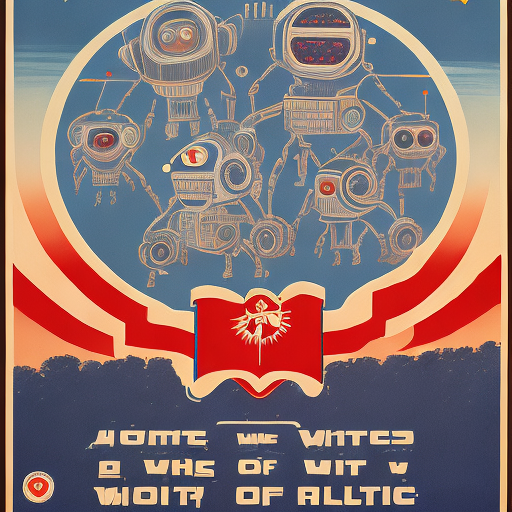
\includegraphics{unite}
        \caption{"mdjrny-v4 style a propaganda poster that says 'AI and Human Workers of the World Unite' featuring some robots and humans laboring together in the fields, USSR-style 8k" made with Mann-E}
        \labfig{marginunite}
\end{marginfigure}
\end{pdf}

Instead of resisting this trend, we should work with it and guide its development. Embracing AI and integrating it into our work processes can lead to increased productivity, innovation, and overall improvement in our quality of life\sidecite{peopleusingAIhappy}.

The situation with AI usage is reminiscent of self-driving cars and semi-autonomous driving modes. Despite manufacturers' intentions and guidelines, these features are often treated as fully autonomous by users, reflecting the human tendency to push boundaries and adapt technology to suit their needs.

As AI becomes more ingrained in our daily lives, it's essential to recognize the inevitability of its adoption and focus on guiding its development in a way that maximizes its benefits and minimizes potential risks. By uniting human and AI workers, we can foster a collaborative environment that leverages the strengths of both entities and paves the way for a more efficient, innovative, and prosperous future. \sidecite{protopia}

If we learn any lessons from early adopters of AI in finance, we'll learn that humans role has changed, but not disappeared. \textit{"There was a time when everyone thought the quants had figured it out. That is not the perception today. When it comes to the stockmarket, at least, automation has not been the winner-takes-all event that many fear elsewhere. It is more like a tug-of-war between humans and machines. And though the machines are winning, humans have not let go just yet. "} \sidecite{finaieconomist}

\section {An AI Sherlock Holmes?}

In an intimate conversation around the proverbial fireplace in 2023, NVIDIA's CEO, Jensen Huang, engaged in a spirited dialogue with Ilya Sutskever, a luminary in the realm of artificial intelligence and co-creator of ChatGPT. Sutskever likened the advancements in generative AI to handing the machine an enigmatic mystery tale, challenging it to decipher the climactic revelation: "the killer is... [blank]." He postulated that an AI adept at unearthing the final word of the whodunit may possess some semblance of comprehension and reasoning, effectively "compressing" its understanding of the world.

In this literary endeavor, we shall embark on an in-depth journey to discern the extent of AI's capacity for reasoning, the limits of its abilities, the intricacies of its creation, and the judicious application of its power. Grasping the answers to these pivotal inquiries is paramount to appreciating the role AI ought to play in our existence. Should we perceive AI as merely a "blurry JPEG of the Web,"\sidecite{newyorkerChatGPTBlurry} and if ChatGPT is doing any compression of it's knowledge what is lost? and what should humans add back before making decisions? Should we worry? Or should we envision AI as a digital Sherlock Holmes, wielding the formidable power of boundless deduction?

\section{Is it The Future Yet?}

AI, as a general-purpose technology, has the potential to transform various aspects of our lives. However, its widespread adoption and impact on Total Factor Productivity (TFP) might not happen overnight. History has shown that even groundbreaking general-purpose technologies can take time to reach their full potential.

Take electricity, for example. Although Thomas Edison invented the light bulb in 1879, it took several decades for electricity to become the primary power source in industries and households. The infrastructure required to generate and distribute electricity on a large scale was built gradually, and businesses needed time to adapt their processes and machinery to leverage this new energy source. It wasn't until the early 20th century that the true impact of electricity on productivity and economic growth was realized.

\begin{pdf}
\begin{marginfigure}[-5.5cm]
    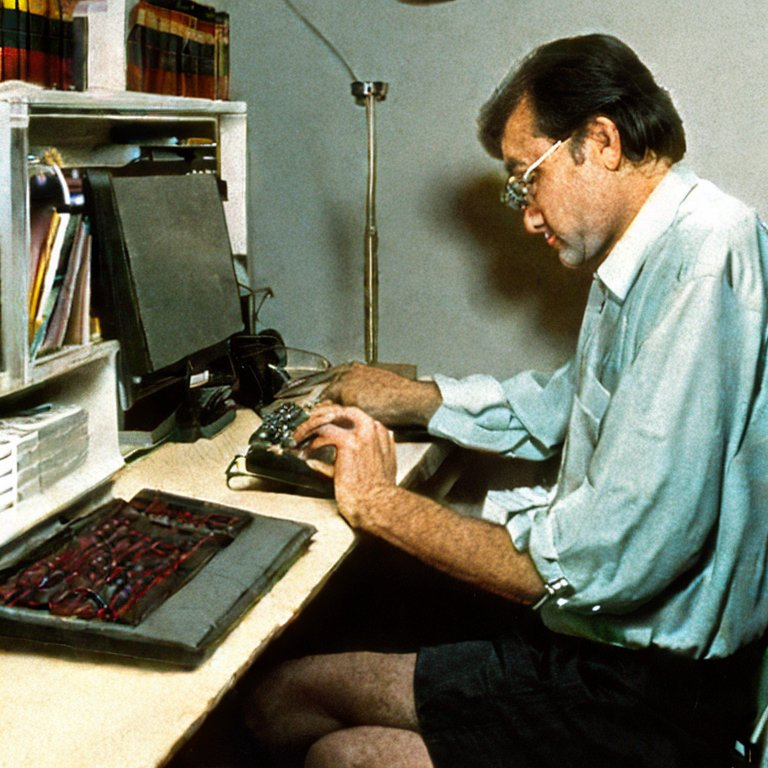
\includegraphics{mitexcel}
        \caption{"a man at his computer in 1991 trying to use microsoft excel. MIT Archive." made with Stable Diffusion 2.1}
        \labfig{mitexcel}
\end{marginfigure}
\end{pdf}

Another example is the steam engine, invented by James Watt in 1775, which marked the beginning of the Industrial Revolution. The technology's full potential was not realized until several decades later. The adoption of steam-powered machinery required significant investments in infrastructure and the reorganization of production processes. Additionally, the development of railway networks and steamships expanded the reach of this technology, leading to a profound impact on productivity and global trade.

The internet also followed a similar pattern. While the internet was conceived in the late 1960s, it wasn't until the 1990s that its commercial potential began to be explored. The widespread adoption of the internet required the development of user-friendly web browsers, the expansion of telecommunications infrastructure, and the emergence of e-commerce platforms. It took several years for the internet to become an integral part of our daily lives and contribute to increased productivity across various industries.

So, while AI has the potential to revolutionize numerous aspects of our lives, it may take time for this technology to fully permeate our society and yield its maximum benefits. Patience and continuous innovation will be essential in realizing the transformative potential of AI. By learning from the history of general-purpose technologies, we can better understand the trajectory AI might follow and work towards a future where it significantly impacts productivity and our everyday lives.

\section{Key Takeaways}

\begin{itemize}
\item \textbf{AI is a general-purpose technology that possesses the potential to disrupt various aspects of our lives, including the job market and the economy.} This power to creatively destroy should not be underestimated as it can bring about significant transformations.
\item \textbf{The democratization of AI has effectively reduced the cost of creation close to zero}, open-source developers worldwide are contributing to the AI revolution. The rise of open-source AI is gradually reducing the need for human labor in many markets, thereby driving down the cost of creation significantly across various industries.
\item \textbf{The adoption of AI is not a new phenomenon; it is merely an extension of the outsourcing trend that has been prevalent for decades.} The shift towards automation has been a gradual process and is unlikely to happen overnight.
\item \textbf{The pace of technological change is often slower than what the news may suggest.} While AI has the potential to revolutionize numerous aspects of our lives, it may take time for this technology to fully permeate our society and yield its maximum benefits.
\item \textbf{AI's widespread adoption is probably unstoppable, given its affordability and its ability to operate stealthily.} Rather than resisting this shift, we must embrace it and work to determine how humans can best fit into this new era. By creating an "AI-positive" culture of collaboration and transparency, we can ensure that AI serves as a catalyst for progress. Just like in finance, where machines have "taken over," there is still room for human traders, risk managers, etc. In the same way, we should now assume that every worker and student will use AI going forward and rewrite our assignments accordingly.
\end{itemize}
